\section{Mixed Criticality Bus Arbiters}

%%%%%%%%%%%%%%%%%%%%%%%%%%%%%%%%%%%%%%%%%
\begin{frame}{Goals of Mixed-Criticality Communication Protocols}

\vspace{-0.3cm}

\visible<1->{
\begin{block}{Resource Utilization}
\begin{itemize}
\item Enable the derivation of tight latency bounds for guaranteed latency traffic
\item Analyzable in terms of schedulability
\end{itemize}
\end{block}
}

\visible<2->{
\begin{block}{Quality of Service}
\begin{itemize}
\item Reduce the average latency of best-effort traffic
\item Not applicable to guaranteed latency traffic
\end{itemize}
\end{block}
}

\visible<3->{
\begin{block}{Scalability}
\begin{itemize}
\item Scale well with the number of bus masters or NoC nodes
\end{itemize}
\end{block}
}

\end{frame}
%%%%%%%%%%%%%%%%%%%%%%%%%%%%%%%%%%%%%%%%%%%%%%%%%%%%%%%
\begin{frame}{TDMA-RR Dual Layer Arbiter}

\vspace{-0.3cm}

\begin{itemize}
\item First layer : TDMA for critical bus masters
\item Second layer : RR for non-critical bus masters
\end{itemize}

\vspace{0.3cm}

\includegraphics<1>[width=\textwidth]{TDMA-RR_Arbiter_Grey.png}
\includegraphics<2>[width=\textwidth]{TDMA-RR_Arbiter.png}

\end{frame}
%%%%%%%%%%%%%%%%%%%%%%%%%%%%%%%%%%%%%%%%%%%%%%%%%%%%%%%
\begin{frame}{Criticality- and Requirement-Aware Bus Arbiter}

\vspace{-0.3cm}

\begin{itemize}
\item \visible<1-> First layer : arbitration between criticality classes
\item \visible<1-> Second layer : arbitration between tasks of the elected criticality class
\item \visible<2-> {Both layers are Weighted Harmonic RR}
\end{itemize}

\visible<2->{
\begin{block}{Weighted Harmonic Round Robin}
\begin{itemize}
\item Bus control granted for 1 request only
\item Each master can get several slots per period
\item Slots are evenly distributed
\end{itemize}
\end{block}
}

\end{frame}

\begin{frame}{CArb - Example}

\vspace{-0.3cm}
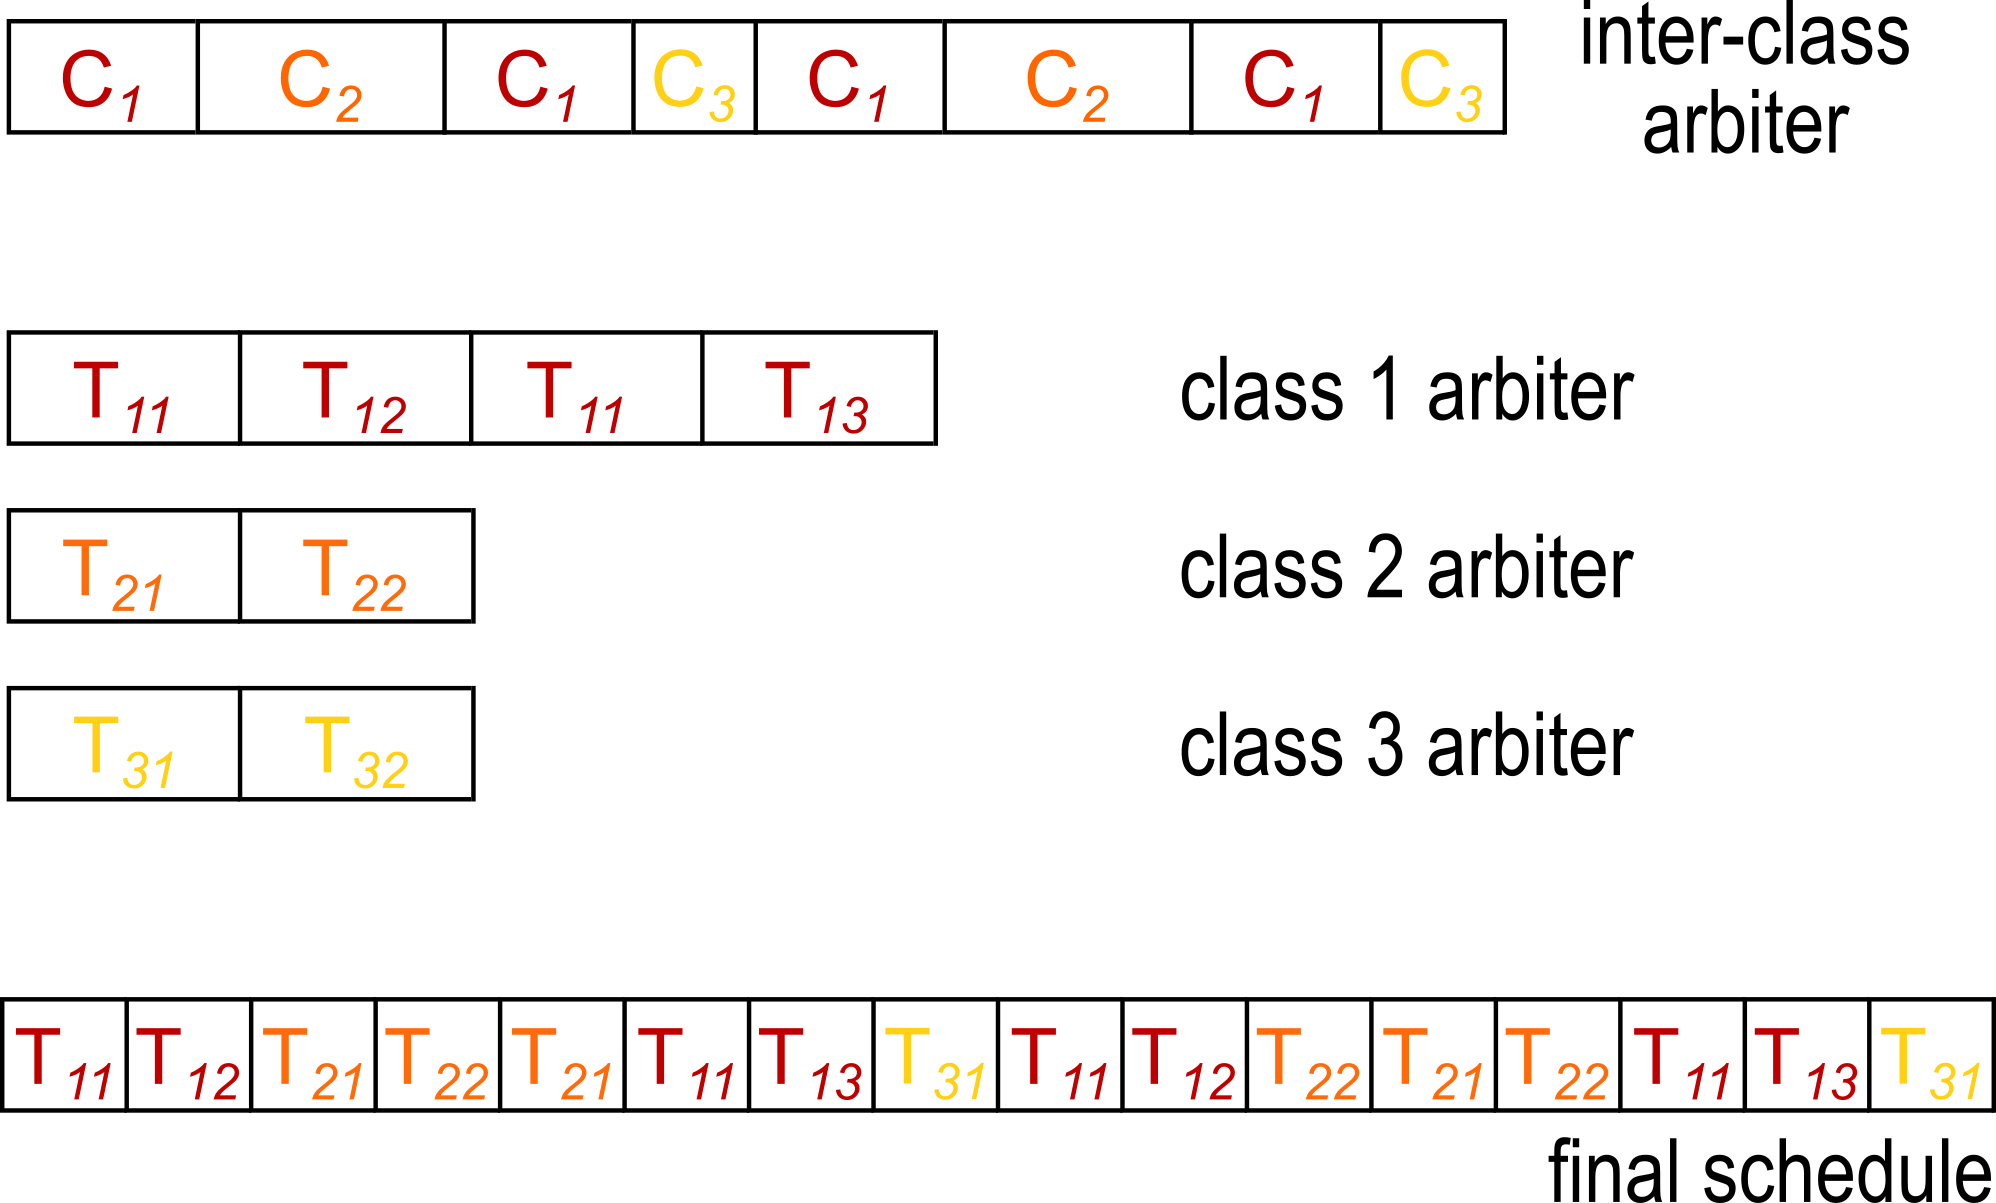
\includegraphics[width=\textwidth]{CArb1.png}

\end{frame}

\begin{frame}{CArb - Arbiter-level Mode Switch}

\visible<1->{
\(\text{WCET}_{total}(\text{T}_{\textit{13}}) < exec\_time(\text{T}_{\textit{13}})\)\\
\(\to\) Drop low-critical tasks, system-wide mode switch
\vspace{0.5 cm}
}

\visible<2->{
\(\text{WCET}_{iso}(\text{T}_{\textit{13}}) < exec\_time(\text{T}_{\textit{13}}) < \text{WCET}_{total}(\text{T}_{\textit{13}})\)\\
\(\to\) Cut interference, arbiter-level mode switch

\begin{center}

\includegraphics[width=0.25\textwidth]{CArb2.png}
\end{center}
}

\visible<3->{
If \(exec\_time(\text{T}_{\textit{13}}) - \text{WCET}_{iso}(\text{T}_{\textit{13}}) < \textit{threshold}\)\\
\(\to\) Cut only part of the interference

\begin{center}

\includegraphics[width=0.90\textwidth]{CArb3.png}
\end{center}
}

\end{frame}


%%% Local Variables:
%%% mode: latex
%%% TeX-master: "slides"
%%% End:
